\chapter{Forcefield Expressions}

A collection of atoms can live quite happily on its own in \progname{}, and can be moved around, rotated, deleted and added to at will. However, if you want to calculate the energy or forces of a collection of atoms (or employ methods that use such quantities) then a description of the interactions between the atoms is required. Creating a suitable $expression$ is the process of taking a system of atoms and generating a prescription for calculating the energy and/or forces arising from these interactions from any standard classical forcefield available.\\

On the way to generating an expression, several preliminary steps are performed:

\begin{enumerate}
	\item Detect molecule patterns for efficient usage of forcefield terms
	\item Augment bonds within (otherwise chemically \qte{correct}) molecules
	\item Find rings and assign aromaticity
	\item Assign atom hybridisation
\end{enumerate}

The first serves to enable the creation of optimal forcefield expressions for systems containing many copies of the same molecules (e.g. liquids), while the last three provide additional data beyond basic topology parameters for use in atom typing. All are performed automatically unless you specifically request them not to be (see Section XXX). The most important of these is the pattern description of the system, without which the expression cannot be created.

\section{Patterns}

Patterns describe systems in terms of their constituent molecular units. For an $N$-component system (a single, isolated molecule is a 1-component system) there are $N$ unique molecule types which are represented as, ideally, a set of $N$ patterns. Forcefield subexpressions can then be created for each pattern and applied to each molecule within it, allowing the expression for the entire system to be compact and efficient. Each pattern contains a list of intramolecular terms (bonds, angles etc.), atom types, and van der Waals parameters for a single molecule that can then be used to calculate the energy and forces of $M$ copies of the molecule.


From the atoms and the basic connectivity between them \progname{} will automatically determine the pattern of systems of arbitrary complexity. The ordering of atoms is important, however, and the atoms belonging to a single molecule must not be interspersed by those from others. In other words, if a bond \qte{crosses an atom} that doesn't belong to the molecule, then the benefits of fine-graining the expression in this way is lost somewhat. There are also many ways to represent the same system of atoms, all of which (from the point of view of the program) are equivalent and will produce the same total energies and atomic forces. Consider the following examples:

\begin{table}
\centering
\begin{tabular}{c c l}
	1. & \multirow{2}{*}{ 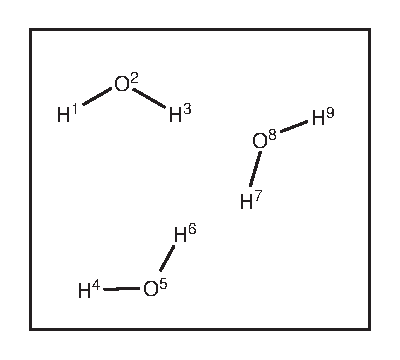
\includegraphics[width=3cm]{figures/pattern1.eps} } &
		Atom Order: H$^1$ O$^2$ H$^3$ H$^4$ O$^5$ H$^6$ H$^7$ O$^8$ H$^9$ \\
		& & Pattern: H$_2$O$(3)$ \\\\\\\\\\\\
	2. & \multirow{2}{*}{ 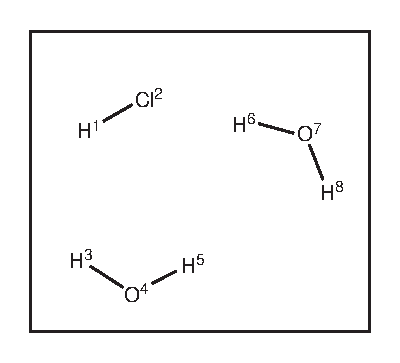
\includegraphics[width=3cm]{figures/pattern2.eps} } &
		Atom Order: H$^1$ Cl$^2$ H$^3$ O$^4$ H$^5$ H$^6$ O$^7$ H$^8$ \\
		& & Pattern: HCl$(1)$ H$_2$O$(2)$ \\\\\\\\\\\\
	3. & \multirow{2}{*}{ 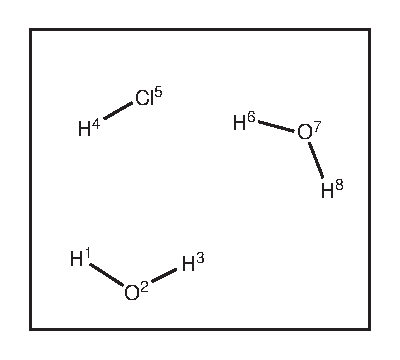
\includegraphics[width=3cm]{figures/pattern3.eps} } &
		Atom Order: H$^1$ O$^2$ H$^3$ H$^4$ Cl$^5$ H$^6$ O$^7$ H$^8$ \\
		& & Pattern: H$_2$O$(1)$ HCl$(1)$ H$_2$O$(1)$ \\\\\\\\\\\\
	4. & \multirow{2}{*}{ 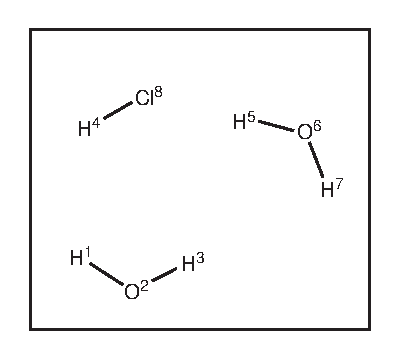
\includegraphics[width=3cm]{figures/pattern4.eps} } &
		Atom Order: H$^1$ O$^2$ H$^3$ H$^4$ H$^5$ O$^6$ H$^7$ Cl$^8$ \\
		& & Pattern: H$_5$O$_2$Cl$(1)$ \\\\\\\\\\\\
\end{tabular}
\end{table}


In 1) the three water molecules are identical with respect to the ordering of the atoms, so our description consists of a single pattern describing one H$_2$O. Obvious, huh? The two-component system illustrated in 2) and 3) is described by two different patterns since, in 3), the two water molecules are \qte{separated} by the hydrogen chloride. Thus, we end up with a three-pattern description to describe the contents of the system as opposed to the optimal two-pattern description, but remember that both are acceptable and will give the same total energies and atomic forces -- only the partitioning of the molecules has changed, and their order is not important (the actual positions of the atoms of course remains constant). This illustrates the point that molecules of the same type need not exist next to each other in terms of the overall atom list, but that the optimal pattern description will not be possible. There are likely to be many possible pattern descriptions for systems, some of which may be useful to employ, and some of which may not be. Take the well-ordered system 1) -- there are four ways to describe the three separate molecules:

\begin{enumerate}
	\item H$_2$O$(3)$
	\item H$_2$O$(1)$ H$_2$O$(1)$ H$_2$O$(1)$
	\item H$_2$O$(2)$ H$_2$O$(1)$
	\item H$_2$O$(1)$ H$_2$O$(2)$
\end{enumerate}

Again, all are equivalent and will give the same energies / forces. Sometimes it is useful to treat individual molecules as separate patterns in their own right since it allows for calculation of interaction energies with the rest of the molecules of the system. \\

Recall that bonds \qte{crossing atoms} will prevent the optimal description of atoms, but now consider that patterns can \qte{cross molecules}. For instance, consider again the example 1) above. Three further (again, reiterating the point, equivalent) ways of writing the pattern description are:

\begin{enumerate}
	\item H$_6$O$_3(1)$
	\item H$_4$O$_2(1)$ H$_2$O$(1)$
	\item H$_2$O$(1)$ H$_4$O$_2(1)$
\end{enumerate}

Here, we have encompassed individual molecular entities into supermolecular groups, and as long as there are no bonds \qte{poking out} of the pattern element, this is perfectly acceptable. Although this coarse-graining is a rather counter-intuitive way of forming patterns, it nevertheless allows them to be created for awkward systems such as that in 4) above. We may write two valid patterns for this arrangement of atoms:

\begin{enumerate}
	\item H$_5$O$_2$Cl$(1)$
	\item H$_2$O$(1)$ H$_3$OCl$(1)$
\end{enumerate}

Note that, when automatically creating patterns, if \progname{} stumbles across a situation like this, it will assume the default pattern of one supermolecule (the whole system of atoms), i.e. X$(1)$ where \qte{X} is all atoms. This will work, but will result in rather inefficient calculations.

\section{Creating the Expression}

For each element in the pattern the required intramolecular terms and atom types are determined for the representative molecule of the element. Atom typing is a complex process and is discussed in detail in Section \ref{sec:typing}. For now, let us assume that each atom in the molecules of each pattern element has been successfully assigned a forcefield type (if this cannot be achieved, then the expression cannot be created). Once \progname{} has convinced itself that every atom has type, a skeleton list of intramolecular terms (currently only bonds, angles, and torsions are supported) necessary to describe the element molecules is constructed and subsequently filled (\qte{fleshed out}) with parameters. These parameters come either from the forcefield associated to the model as a whole, or from individual forcefields associated to individual elements of the pattern (see Section XX), based on the assigned types of the atoms. If one or more suitable terms cannot be found in the forcefield(s), energies and forces cannot be calculated. Admittedly, this is a little Draconian, and will be addressed in a future release. \\

Once constructed, a complete expression persists until a change is made to the model which is potentially invalidates it. For example, moving atoms around is acceptable, but changes in bonding are not. Nor is adding or deleting atoms, since this obviously requires regeneration of the pattern description. In such cases, the expression is marked as out-of-date and will be automatically recreated when it is next required.
